\documentclass[11pt]{article}
\usepackage[scaled=0.92]{helvet}
\usepackage{geometry}
\geometry{letterpaper,tmargin=1in,bmargin=1in,lmargin=1in,rmargin=1in}
\usepackage[parfill]{parskip} % Activate to begin paragraphs with an empty line rather than an indent %\usepackage{graphicx}
\usepackage{amsmath,amssymb, mathrsfs, dsfont}
\usepackage{tabularx}
\usepackage[font=footnotesize,labelfont=bf]{caption}
\usepackage{graphicx}
\usepackage{xcolor}
%\usepackage[linkbordercolor ={1 1 1} ]{hyperref}
%\usepackage[sf]{titlesec}
\usepackage{natbib}
\usepackage{../../Tianpei_Report}

%\usepackage{appendix}
%\usepackage{algorithm}
%\usepackage{algorithmic}

%\renewcommand{\algorithmicrequire}{\textbf{Input:}}
%\renewcommand{\algorithmicensure}{\textbf{Output:}}



\begin{document}
\title{Lecture 6: The Gauss-Bonnet Theorem and its Applications}
\author{ Tianpei Xie}
\date{Oct. 13th., 2022}
\maketitle
\tableofcontents
\newpage
\section{The Gauss-Bonnet Theorem}
\begin{itemize}
\item The \emph{\textbf{Gauss-Bonnet theorem}} is probably the \emph{\textbf{deepest theorem}} in the differential geometry of surfaces. A first version of this theorem was presented by Gauss in a famous paper and deals with \emph{\textbf{geodesic triangles}} on surfaces (that is, \emph{triangles} whose sides are \emph{arcs} of \emph{geodesics}). 

\begin{figure}[htb]
\centering
\begin{minipage}{1\linewidth}
 \centerline{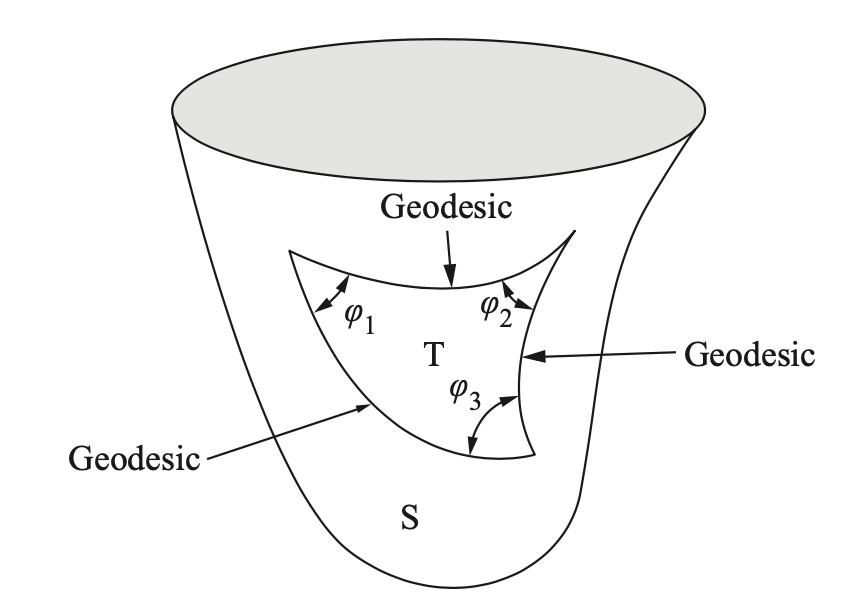
\includegraphics[scale = 0.5]{geodesic_triangle.png}}
\end{minipage}
\caption{\scriptsize
\textbf{A geodesic triangle is formed by three joined geodesic arcs on the surface}}
\label{fig: geodesic_triangle}
\end{figure}


\item Roughly speaking, it asserts that the \emph{\textbf{excess}} over $\pi$ of the \textbf{\emph{sum} of the \emph{interior angles}} $\varphi_1$, $\varphi_2$, $\varphi_3$ of a geodesic triangle $T$ \textbf{is equal to} the \emph{integral} of the \emph{\textbf{Gaussian curvature}} $\mb{K}$ over $T$; that is (Fig. \ref{fig: gauss_bonnet}),
\begin{align*}
\sum_{i=1}^{3}\varphi_i - \pi &= \iint_{T} \mb{K} d\sigma
\end{align*}

\begin{figure}[htb]
\centering
\begin{minipage}{1\linewidth}
 \centerline{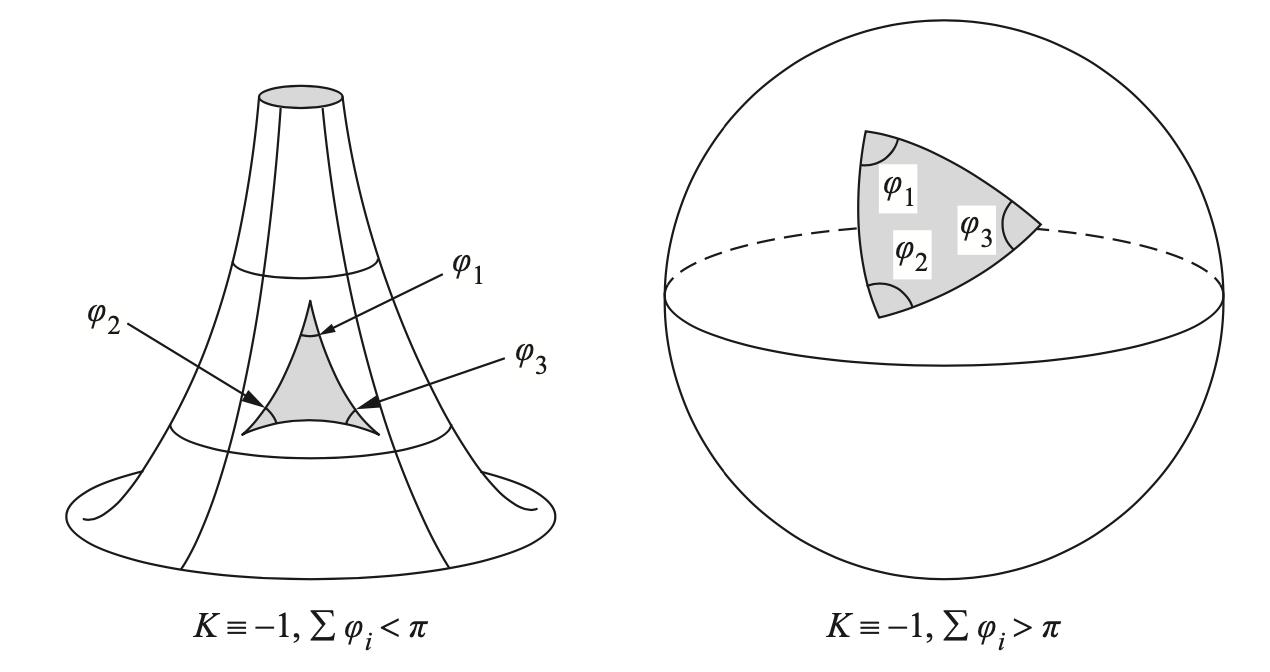
\includegraphics[scale = 0.5]{gauss_bonnet.png}}
\end{minipage}
\caption{\scriptsize
\textbf{A surprising fact is that the sum of interior angles of a triangle on surface is not necessarily $\pi$, and it depends on the intrinsic geometry of surface only. \citep{do1976differential}}}
\label{fig: gauss_bonnet}
\end{figure}

\item The extension of the theorem to a region bounded by a nongeodesic simple curve is due to O. Bonnet. To extend it even further, say, to compact surfaces, some topological considerations will come into play. Actually, one of the most important features of the Gauss-Bonnet theorem is that it provides a remarkable relation between the topology of a compact surface and the integral of its curvature.
\end{itemize}
\subsection{The Prerequisites for Proof of Gauss-Bonnet Theorem (Local)}
\begin{itemize}
\item \begin{definition}
Let $\alpha: [0, 1] \rightarrow \cS$ be a \emph{continuous} map from the closed interval $[0, 1]$ into the \emph{regular surface} $\cS$. We say that $\alpha$ is a \emph{\textbf{simple}}, \emph{\textbf{closed}}, \emph{\textbf{piecewise regular}}, \emph{parametrized curve} if
\begin{enumerate}
\item (\emph{\textbf{closedness}}) $\alpha(0) = \alpha(1).$
\item (\emph{\textbf{no self-intersection}}) $ t_1 \neq t_2, \; t_1, t_2 \in [0,1)$, implies that $\alpha(t_1) \neq \alpha(t_2).$
\item (\emph{\textbf{tangent line well defined except for a finite number of points}})\\ 
There exists a \emph{subdivision} 
\begin{align*}
0= t_0 < t_1 < \ldots < t_k < t_{k+1} = l,
\end{align*} of $(0,1]$ such that $\alpha$ is \emph{\textbf{differentiable}} and \emph{regular} in each $(t_i,t_{i+1})$, $i = 0,\ldots,k$.
\end{enumerate}
\end{definition}

\item The points $\alpha(t_i), i = 0, \ldots, k$, are called the \emph{\textbf{vertices}} of $\alpha$ and the \emph{traces} $\alpha([t_i , t_{i+1}])$ are called the \emph{\textbf{regular arcs}} of $\alpha$. It is usual to call the trace $\alpha([0, 1])$ of $\alpha$, a \emph{\textbf{closed piecewise regular curve}}.

\item By the condition of \emph{regularity}, for each \emph{vertex} $\alpha(t_i)$ there exist the \emph{limit} from \emph{the left}, i.e., for $t < t_i$,
\begin{align*}
\lim_{t \rightarrow t_i}\alpha'(t) &=  \alpha'(t_i - 0) \neq 0, 
\end{align*}
and the \emph{limit} from the right, i.e., for $t > t_i$, 
\begin{align*}
\lim_{t \rightarrow t_i}\alpha'(t) &=  \alpha'(t_i + 0) \neq 0, 
\end{align*}

\begin{figure}[htb]
\centering
\begin{minipage}{1\linewidth}
 \centerline{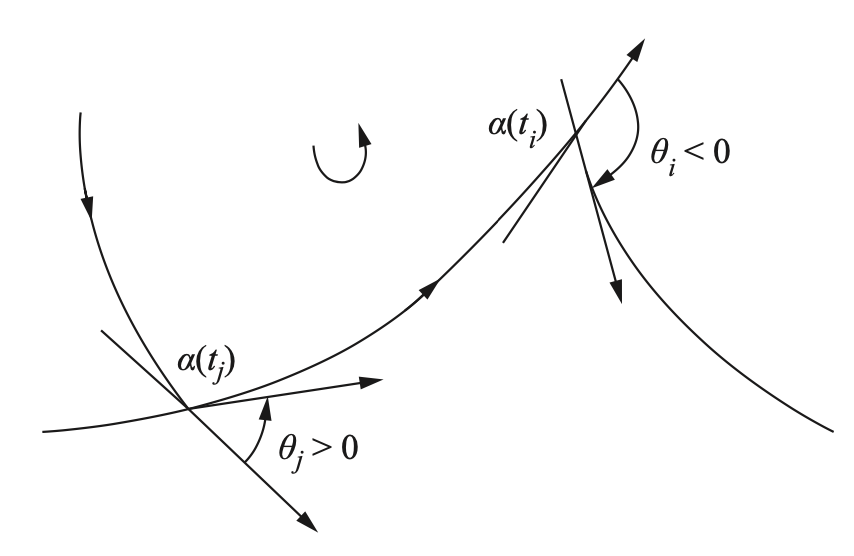
\includegraphics[scale = 0.5]{gauss_bonnet_fig_2.png}}
\end{minipage}
\caption{\scriptsize
\textbf{$\alpha(t_i)$ is not a cusp \citep{do1976differential}}}
\label{fig: gauss_bonnet_fig_2}
\end{figure}

\item Assume now that $\cS$ is \emph{\textbf{oriented}} and let $\abs{\theta_i}$, $0 \le \abs{\theta_i} < \pi$, be the \emph{\textbf{smallest determination}} of the angle from $\alpha'(t_i - 0)$ to $\alpha'(t_i + 0)$. If $\abs{\theta_i} \neq \pi$, we give $\theta_i$ the \emph{\textbf{sign}} of the \emph{determinant} $(\alpha'(t_i - 0), \alpha'(t_i + 0), \mb{N})$. This means that if the vertex $\alpha(t_i)$ is \textbf{not a "cusp"} (Fig. \ref{fig: gauss_bonnet_fig_2}), the \emph{\textbf{sign}} of $\theta_i$ is given by the \emph{orientation} of $\cS$. The \emph{\textbf{signed angle}} $\theta_i$, $-\pi < \theta_i < \pi$, is called \emph{\textbf{the external angle}} at the vertex $\alpha(t_i)$.

In the case that $\alpha(t_i)$ \textbf{is a cusp}, i.e., $\abs{\theta_i} = \pi$, we choose the \emph{sign} of $\theta_i$ as follows. Let the closed simple curve $\alpha$ be \emph{contained} in the \emph{image} of a \emph{\textbf{conformal} parametrization with a given \textbf{orientation}} and assume that $\alpha(t_i)$ is a cusp. Choose coordinate axis $x0y$, with $\alpha(t_i) = 0,$ in the given orientation, and assume further that the part of $\alpha$ arriving at $\alpha(t_i)$ is point towards the negative part of the axix $0x$ 
(and of course the part of $\alpha$ leaving at $\alpha(t_i)$ is point towards the positive part of the axix $0x$).

For small $\epsilon > 0$, the part of  $\alpha$  arriving at $\alpha(t_i)$, and near it, is given by a function $f(x) = y$ for $0 < x < \epsilon$, and the part of $\alpha$ leaving at $\alpha(t_i)$, and near it, is given by a function $g(x) = y$ for $0 < x < \epsilon$. If $f >0$ and $g  < 0$, then we set $\theta(t_i) = \pi$; if $f < 0$ and $g > 0$, then we set $\theta(t_i) = -\pi$.

\begin{figure}[htb]
\centering
\begin{minipage}{1\linewidth}
 \centerline{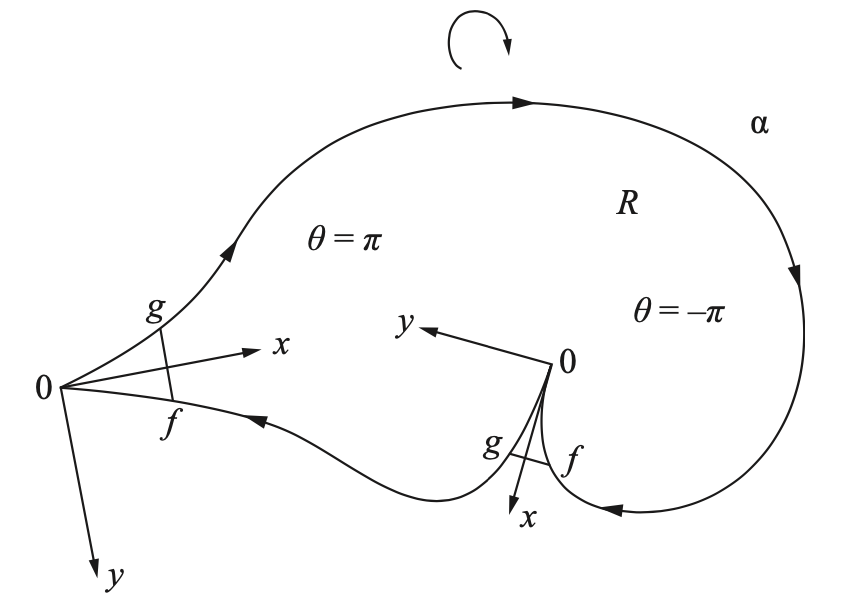
\includegraphics[scale = 0.5]{gauss_bonnet_fig_3.png}}
\end{minipage}
\caption{\scriptsize
\textbf{$\alpha(t_i)$ is a cusp \citep{do1976differential}}}
\label{fig: gauss_bonnet_fig_3}
\end{figure}


\item Let $\alpha: [0, 1] \rightarrow \mb{x}(U) \subset \cS$ be a \emph{simple, closed, piecewise regular, parametrized curve} with vertices $\alpha(t_i)$ and external angles $\theta_i$, $i = 0, \ldots, k$.

Let $\varphi_i: [t_i, t_{i+1}] \rightarrow \bR$ be differentiable functions with measure at each $t \in [t_i, t_{t+1}]$ the positive angle from $\mb{x}_{u}$ to $\alpha'(t)$. 

The following topological fact is
\begin{theorem} (Theroem of \textbf{Turning Tangents})\label{thm: turning_tangents}\\
With above notations, we have for the plane curves,
\begin{align*}
\sum_{i=1}^{k}\paren{\varphi_i(t_{i+1}) - \varphi_{i}(t_{i})} + \sum_{i=1}^{k}\theta_i &= \pm 2\pi
\end{align*}
\end{theorem}
The theorem states that the \emph{total variation} of the angle of tangent vector to $\alpha$ with a given direction plus the "jumps" at the vertices is equal to $2\pi$.

\item \begin{definition}
Let $\cS$ be an \emph{\textbf{oriented surface}}. A region $\cR \subset \cS$ (union of a \emph{connected open set} with its \emph{boundary}) is called a \emph{\textbf{simple region}} if $\cR$ is \emph{\textbf{homeomorphic}} to a \emph{\textbf{disk}} and the \emph{\textbf{boundary}} $\partial \cR$ of $\cR$ is the \emph{trace} of a \emph{simple, closed, piecewise regular, parametrized curve} $\alpha: I \rightarrow \cS$. 
\end{definition}

\item \begin{definition}
We say then that $\alpha$ is \emph{\textbf{positively oriented}} if for each $\alpha(t)$, belonging to a \emph{regular arc}, the \emph{\textbf{positive orthogonal basis}} $\set{\alpha'(t), h(t)}$ satisfies the condition that $h(t)$ "\emph{points toward}" $\cR$; more precisely, for any curve $\beta: I \rightarrow \cR$ with $\beta(0) = \alpha(t)$ and $\beta'(0)  \neq  \alpha'(t)$, we have that 
$\inn{\beta'(0)}{h(t)} > 0$.
\end{definition}

\begin{figure}[htb]
\centering
\begin{minipage}{1\linewidth}
 \centerline{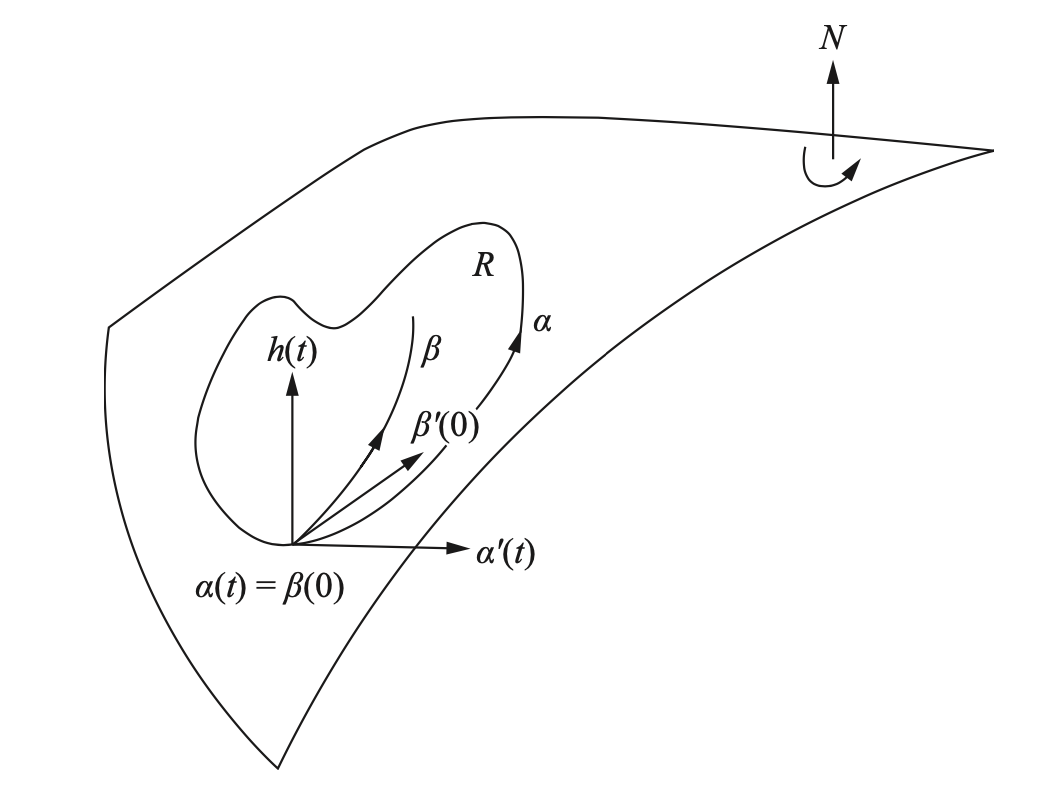
\includegraphics[scale = 0.5]{positive_oriented_boundary_curve.png}}
\end{minipage}
\caption{\scriptsize
\textbf{A positive oriented boundary curve \citep{do1976differential}}}
\label{fig: positive_oriented_boundary_curve}
\end{figure}


Intuitively, this means that if one is walking on the curve $\alpha$ in the \emph{positive direction} and with one’s \emph{head pointing} to $\mb{N}$, then the region $\cR$ remains to the \emph{\textbf{left}} (Fig. \ref{fig: positive_oriented_boundary_curve}). It can be shown that \emph{one of the two possible orientations} of $\alpha$ makes it \emph{positively oriented}.

\item Now let $\mb{x}: U \subset \cR^2 \rightarrow \cS$ be a \emph{\textbf{parametrization}} of $\cS$ \emph{compatible} with its \emph{orientation} and let $\cR \subset \mb{x}(U)$ be a \emph{\textbf{bounded region}} of $\cS$. If $f$ is a \emph{\textbf{differentiable}} function on $\cS$, then it is easily seen that the integral
\begin{align*}
\iint_{\mb{x}^{-1}(\cR)} f(u, v)\,\sqrt{EG - F^2} du\,dv
\end{align*} \emph{\textbf{does not depend on the parametrization}} $\mb{x}$, chosen in the class of \emph{orientation} of $\mb{x}$.

This integral has, therefore, a \emph{\textbf{geometrical meaning}} and is called the \emph{\textbf{integral of $f$ over the region $\cR$}}. It is usual to denote it by
\begin{align*}
\iint_{\cR}f\,d\sigma
\end{align*}
\end{itemize}
\subsection{The Gauss-Bonnet Theorem (Local)}
\begin{itemize}
\item We states the local version of the Gauss-Bonnet Theorem
\begin{theorem}\label{thm: gauss_bonnet_local}  (\textbf{Gauss-Bonnet Theorem (Local)}) \citep{do1976differential}\\
Let $\mb{x}: U \rightarrow \cS$ be an \textbf{isothermal parametrization} (i.e., $F = 0, E = G = \lambda^2(u, v)$) of an oriented surface $\cS$, where $U \subset \cR^2$ is \textbf{homeomorphic} to an \textbf{open disk} and $\mb{x}$ is compatible with the orientation of $\cS$. Let $\cR \subset \mb{x}(U)$ be a \textbf{simple region} of $\cS$ and let $\alpha: I \rightarrow \cS$ be such that  $\partial \cR = \alpha(I)$. Assume that $\alpha$ is \textbf{positively oriented}, parametrized by arc length $s$, and let $\alpha(s_0),\ldots, \alpha(s_k)$ and $\theta_0,\ldots,\theta_k$ be, respectively, the vertices and the \textbf{external angles} of $\alpha$. Then
\begin{align}
\sum_{i=1}^{k}\int_{s_{i}}^{s_{i+1}}k_{g}(s)ds + \iint_{\cR}\mb{K}d\sigma + \sum_{i=1}^{k}\theta_{i} &= 2\pi \label{eqn: gauss_bonnet}
\end{align} where $k_g(s)$ is the \textbf{geodesic curvature} of the regular arcs of $\alpha$ and $\mb{K}$ is the
\textbf{Gaussian curvature} of $\cS$.
\end{theorem}

\begin{remark}
The restriction that the region $\cR$ be contained in the image set of an isothermal parametrization is needed only to simplify the proof and to be able to use the theorem of turning tangents. As we shall see later (Corollary 1 of the global Gauss-Bonnet theorem) the above result still holds for any simple region of a regular surface. This is quite plausible, since Eq. \eqref{eqn: gauss_bonnet} does not involve in any way a particular parametrization. \citep{do1976differential}
\end{remark}

\begin{proof}
Let $u = u(s)$, $v = v(s)$ be the expression of $\alpha$ in the parametrization $\mb{x}$. Recall that the geodesic curvature can be represented in terms of coefficients of the first fundamental form:
\begin{align*}
k_{g}(s) &= \frac{1}{\sqrt{2\,E\,G}}\set{G_{u}\frac{dv}{ds} - E_{v}\frac{du}{ds} } + \frac{d\varphi_{i}}{ds}
\end{align*} where $\varphi_i = \varphi_i(s)$ is a differentiable function which measures the positive angle from $\mb{x}_u$ to $\alpha'(s)$ in $[s_i,s_{i+1}]$. By integrating the above expression in every interval $[s_i,s_{i+1}]$ and adding up the results,
\begin{align*}
\sum_{i=1}^{k}\int_{s_{i}}^{s_{i+1}}k_{g}(s)ds &= \sum_{i=1}^{k}\int_{s_{i}}^{s_{i+1}}\frac{1}{\sqrt{2\,E\,G}}\set{G_{u}\frac{dv}{ds} - E_{v}\frac{du}{ds} }ds + \sum_{i=1}^{k}\int_{s_{i}}^{s_{i+1}}\frac{d\varphi_{i}}{ds}ds
\end{align*}

To compute the first term, we use \emph{the Gauss-Green theorem} in the $uv$ plane which states the following: 
If $P(u,v)$ and $Q(u,v)$ are differentiable functions in a simple region $A \subset \cR^2$, the boundary of which is given by $u = u(s)$, $v = v(s)$, then
\begin{align*}
\sum_{i=1}^{k}\int_{s_{i}}^{s_{i+1}}\paren{P\frac{du}{ds} + Q\frac{dv}{ds}}ds &= \iint_{A} \paren{\partdiff{Q}{u} - \partdiff{P}{v}}du\,dv
\end{align*}
Let $Q:= G_{u}/\sqrt{2\,E\,G}$ and $P:= -E_{v}/\sqrt{2\,E\,G}$, it follows that the first term 
\begin{align*}
\sum_{i=1}^{k}\int_{s_{i}}^{s_{i+1}}\frac{1}{\sqrt{2\,E\,G}}\set{G_{u}\frac{dv}{ds} - E_{v}\frac{du}{ds} }ds
&= \iint_{\mb{x}^{-1}(\cR)}\set{\paren{\frac{E_{v}}{\sqrt{2\,E\,G}}}_{v} + \paren{\frac{G_{u}}{\sqrt{2\,E\,G}}}_{u} } du\,dv
\end{align*}

To be able to use \emph{the theorem of turning tangents}, we must assume that our parametrization is \textbf{isothermal}, that is, in addition to $F = 0$, we have that $E = G = \lambda(u, v) > 0$. In this case, 
\begin{align}
\set{\paren{\frac{E_{v}}{\sqrt{2\,E\,G}}}_{v} + \paren{\frac{G_{u}}{\sqrt{2\,E\,G}}}_{u} } &= \frac{1}{2}\set{\paren{\frac{\lambda_{v}}{\lambda}}_{v} + \paren{\frac{\lambda_{u}}{\lambda}}_{u}} \nonumber\\
&= \frac{1}{2\lambda}\set{(\log \lambda)_{v,v} + (\log \lambda)_{u,u}}\lambda \nonumber\\
&= \frac{1}{2\lambda}\paren{\Delta \log \lambda}\lambda = -\mb{K}\lambda \label{eqn: gauss_bonnet_first_term}
\end{align} where, in the last equality we have used the Exercise 2 of Section 4-3 in \citep{do1976differential}. By integrating the first term expression in the domain of the coordinate neighborhood, we obtain
\begin{align*}
\sum_{i=1}^{k}\int_{s_{i}}^{s_{i+1}}\frac{1}{\sqrt{2\,E\,G}}\set{G_{u}\frac{dv}{ds} - E_{v}\frac{du}{ds} }ds &= - \iint_{\cR}\mb{K}\lambda \;du\,dv
\end{align*}

On the other hand, by the \emph{theorem of turning tangents}, the second term is
\begin{align*}
\sum_{i=1}^{k}\int_{s_{i}}^{s_{i+1}}\frac{d\varphi_{i}}{ds}ds &= \sum_{i=1}^{k}\paren{\varphi_{i}(s_{i+1}) - \varphi_{i}(s_{i})}\\
&= \pm 2\pi - \sum_{i=1}^{k}\theta_i
\end{align*}

Since the curve $\alpha$ is positively oriented, the sign should be plus, as can easily be seen in the particular case of the circle in a plane. By putting these facts together, we obtain
\begin{align*}
\sum_{i=1}^{k}\int_{s_{i}}^{s_{i+1}}k_{g}(s)ds + \iint_{\cR}\mb{K}d\sigma + \sum_{i=1}^{k}\theta_{i} &= 2\pi
\end{align*}\qed
\end{proof}

\begin{figure}[htb]
\centering
\begin{minipage}{1\linewidth}
 \centerline{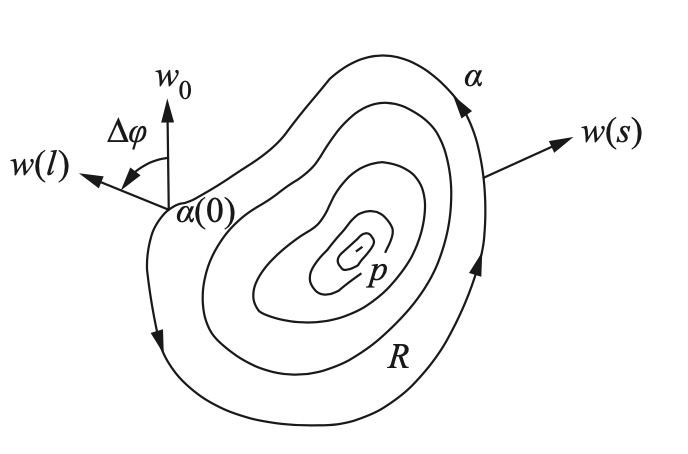
\includegraphics[scale = 0.5]{gaussian_curvature_angle_diff.png}}
\end{minipage}
\caption{\scriptsize
\textbf{An alternative geometrical interpretation of Gaussian curvature using parallelism. \citep{do1976differential}}}
\label{fig: gaussian_curvature_angle_diff}
\end{figure}


\item \begin{remark}
It is seen that the techniques used in the proof of this theorem may also be used to give an interpretation of the \underline{\textbf{Gaussian curvature}} in terms of \underline{\emph{\textbf{parallelism}}}. 

Let $\mb{x}: U \rightarrow \cS$ be an \textbf{isothermal parametrization} (i.e., $F = 0, E = G = \lambda^2(u, v)$) at point $p \in \cS$ and let $\cR \subset \mb{x}(U)$ be a \emph{simple} region \emph{without vertices}, containing $p$ in its interior. Let $\alpha: [0,1] \rightarrow \mb{x}(U)$ be a curve parametrized by arc length $s$ such that the trace of $\alpha$ is the boundary of $\cR$. Let $\mb{w}_0$ be a unit vector \emph{\textbf{tangent}} to $\cS$ at $\alpha(0)$ and let $\mb{w}(s)$, $s \in [0, 1]$, be the \emph{\textbf{parallel transport}} of $\mb{w}_0$ \emph{along} $\alpha$ (Fig. 4-28). By using representation of algebraic value in terms of $E,F,G$ and the Gauss-Green theorem in the $uv$ plane, we obtain
\begin{align*}
 0 &= \int_{0}^{1}\frac{D\mb{w}}{ds}\,ds \\
 &= \int_{0}^{1} \frac{1}{2\sqrt{EG}}\set{G_{u}\frac{dv}{ds} - E_{v}\frac{du}{ds}}ds +  \int_{0}^{1}\frac{d\varphi}{ds}ds\\
 &= -\iint_{\cR}\mb{K}d\sigma + \varphi(1) - \varphi(0)
\end{align*} where $\varphi = \varphi(s)$ is a differentiable \emph{determination} of the \emph{\textbf{angle}} from $\mb{x}_u$ to $\mb{w}(s)$.

It follows that $\varphi(1) - \varphi(0) = \Delta \varphi$ is given by
\begin{align}
 \Delta \varphi &= \iint_{\cR}\mb{K}d\sigma \label{eqn: gaussian_curvature_angle_diff}
\end{align}

Now, $\Delta \varphi$ does not depend on the choice of $\mb{w}_0$, and it follows from the expression above that $\Delta \varphi$ does not depend on the choice of $\alpha(0)$ either. By taking the limit
\begin{align*}
\lim_{\cR \rightarrow p}\frac{\Delta \varphi}{A(\cR)} &= \mb{K}(p),
\end{align*} where $A(\cR)$ denotes the \emph{\textbf{area}} of the region $\cR$, we obtain the desired interpretation of $\mb{K}$.
\end{remark}
\end{itemize}
\subsection{The Prerequisites for Proof of  Gauss-Bonnet Theorem (Global)}
\begin{itemize}
\item \begin{definition}
Let $\cS$ be a \emph{\textbf{regular surface}}. A \emph{connected} region $\cR \subset \cS$ is said to be \emph{\textbf{regular}} if $\cR$ is \emph{\textbf{compact}} and its \emph{boundary} $\partial \cR$ is the \emph{\textbf{finite union}} of (simple) \emph{closed} \emph{piecewise} \emph{regular curves} which do  \emph{\textbf{not intersect}} (the region in Fig. \ref{fig: gauss_bonnet_regular_surface} (a) is regular, but that in Fig. \ref{fig: gauss_bonnet_regular_surface} (b) is not). For convenience, we shall consider a compact surface as a regular region, the boundary of which is empty.
\end{definition}

\begin{figure}[htb]
\centering
\begin{minipage}{1\linewidth}
 \centerline{\includegraphics[scale = 0.5]{gauss_bonnet_regular_surface.png}}
\end{minipage}
\caption{\scriptsize
\textbf{(a) A regular region (b) Not a regular region. \citep{do1976differential}}}
\label{fig: gauss_bonnet_regular_surface}
\end{figure}

\item A simple region which has only three vertices with external angles $\alpha_i \neq 0$, $i = l, 2, 3$, is called a \emph{\textbf{triangle}}.

\item A \emph{\textbf{triangulation}} of a regular region $\cR \subset \cS$ is a finite family $J$ of triangles $T_i$, $i= 1,\ldots,n$, such that
\begin{enumerate}
\item $\bigcup_{i=1}^{n}T_{i} = \cR$
\item If $T_i \cap T_j  \neq \emptyset$, then $T_i \cap T_j$ is either a common edge of $T_i$ and $T_j$ or a
common vertex of $T_i$ and $T_j$.
\end{enumerate}

\item Given a triangulation $J$ of a regular region $\cR \subset \cS$  of a surface $\cS$, we shall denote by $F$ the \emph{number of triangles (\textbf{faces})}, by $E$ \emph{the number of sides (\textbf{edges})}, and by $V$ \emph{the number of \textbf{vertices} of the triangulation}. The number
\begin{align*}
F - E + V &= \chi
\end{align*} is called \emph{\textbf{the Euler-Poincar\'e characteristic of the triangulation}}.

\item \begin{proposition}
\textbf{Every regular region} of a regular surface admits a \textbf{triangulation}.
\end{proposition}

\begin{figure}[htb]
\centering
\begin{minipage}{1\linewidth}
 \centerline{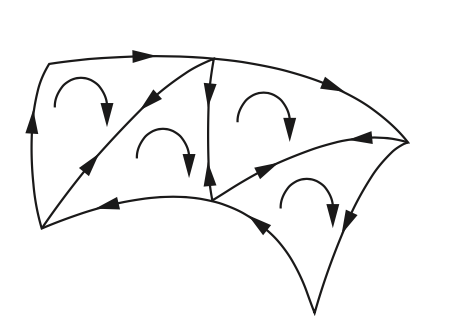
\includegraphics[scale = 0.5]{triangulation.png}}
\end{minipage}
\caption{\scriptsize
\textbf{Triangulation and orientation. \citep{do1976differential}}}
\label{fig: triangulation}
\end{figure}


\item \begin{proposition}
Let $\cS$ be an oriented surface and $\set{\mb{x}_{\alpha}}$, $\alpha \in A$, \textbf{a family of parametrizations} compatible with the orientation of $\cS$. Let $\cR \subset \cS$ be a \textbf{regular region} of $\cS$. Then there is a \textbf{triangulation} of $J$ of $\cR$ such that every triangle $T \in J$ is contained in some coordinate neighborhood of the family $\set{\mb{x}_{\alpha}}$. Furthermore, if the \textbf{boundary} of \textbf{every triangle} of $J$ is \textbf{positively oriented}, \textbf{adjacent} triangles determine \textbf{opposite orientations} in the common edge.
\end{proposition}

\item \begin{proposition}
If $\cR \subset \cS$ is a regular region of a surface $\cS$, the \textbf{the Euler-Poincar\'e characteristic} does \textbf{not} depend on the \textbf{triangulation} of $\cR$. It is convenient, therefore, to denote it by $\chi(\cR)$
\end{proposition}
The latter proposition shows that the \emph{Euler-Poincar\'e characteristic} is a \emph{\textbf{topological invariant}} of the \emph{regular region} $\cR$. For the sake of the applications of the Gauss-Bonnet theorem, we shall mention the important fact that this invariant allows a \textbf{\emph{topological classification}} of the \emph{\textbf{compact} surfaces} in $\bR^3$.

$\chi(\cR) = 2$ for sphere; $\chi(\cR) = 0$ for torus and the $n$-torus is $-2(n-1)$

\begin{figure}[htb]
\centering
\begin{minipage}{1\linewidth}
 \centerline{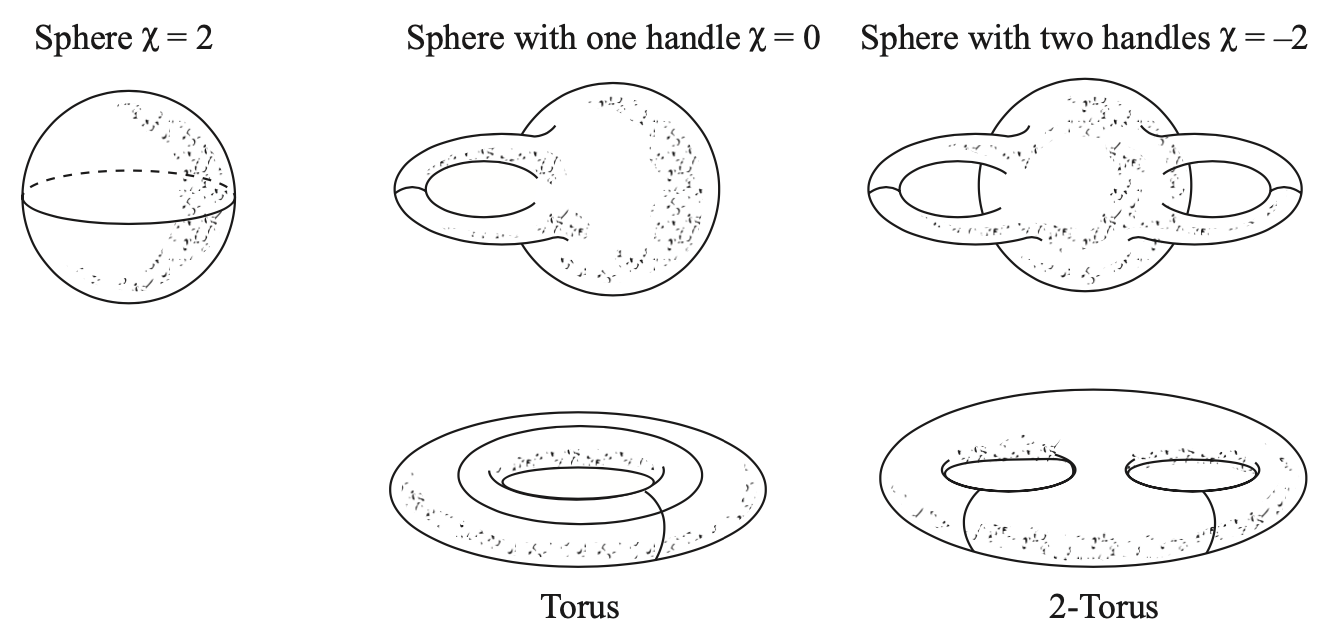
\includegraphics[scale = 0.5]{genus_surface.png}}
\end{minipage}
\caption{\scriptsize
\textbf{Euler-Poincar\'e characteristic $\chi(\cS)$ \citep{do1976differential}}}
\label{fig: genus_surface}
\end{figure}

\item \begin{proposition}
Let $\cS \subset \bR^3$ be a \textbf{compact} connected surface; then one of the values $2,0,-2,\ldots, -2n, \ldots$ is assumed by the Euler-Poincaré characteristic $\chi(\cS)$. Furthermore, if $\cS' \subset \bR^3$ is another compact surface and $\chi(\cS) = \chi(\cS')$, then $\cS$ is \textbf{homeomorphic} to $\cS'$.
\end{proposition}



\item In other words, every compact connected surface $\cS \subset \bR^3$ is \emph{\textbf{homeomorphic}} to a \textbf{\emph{sphere}} with a certain number $g$ of \emph{\textbf{handles}}. The number
\begin{align*}
g &= \frac{2-\chi(\cS)}{2}
\end{align*} is called the \emph{\textbf{genus}} of $\cS$.

\item Let $\cS \subset \bR^3$ be a regular region of an oriented surface $\cS$ and let $J$ be a triangulation of $\cR$ such that every triangle $T_j \in J, j = 1,\ldots,k$, is contained in a coordinate neighborhood $\mb{x}_j (U_j)$ of \emph{\textbf{a family of parametrizations}} $\set{\mb{x}_{\alpha}}$, $\alpha \in A$, compatible with the orientation of $\cS$. Let $f$ be a \emph{differentiable} function on $\cS$. The following proposition shows that it makes sense to talk about the integral of $f$ over the region $\cR$.

\begin{proposition}\label{prop: area_integral}
With the above notation, the sum 
\begin{align*}
\sum_{j=1}^{k}\iint_{\mb{x}_{j}^{-1}(T_{j})}f(u_j, v_j)\sqrt{E_j\,G_j - F_j^2}\; du_j\,dv_j
\end{align*}
does \textbf{not depend} on the \textbf{triangulation} $J$ or on the family $\set{\mb{x}_{j}}$ of \textbf{parametrizations} of $\cS$.
\end{proposition}

This sum has, therefore, a geometrical meaning and is called the \emph{\textbf{integral of $f$ over the regular region $\cR$}}. It is usually denoted by
\begin{align*}
\iint_{\cR} f\;d\sigma
\end{align*}
\end{itemize}

\subsection{The Gauss-Bonnet Theorem (Global)}
\begin{itemize}
\item 
\begin{theorem}\label{thm: gauss_bonnet_global} (\textbf{Gauss-Bonnet Theorem (Global)}) \citep{do1976differential}\\
Let $\cR \subset \cS$  be a \textbf{regular region} of an oriented surface and let $C_1,\ldots, C_n$ be the closed, simple, piece-wise regular curves which form the \textbf{boundary} $\partial \cR$ of $\cR$. Suppose that each $C_i$ is positively oriented and let $\theta_0,\ldots,\theta_p$ be the set of \textbf{all external angles of the curves} $C_1,\ldots, C_n$. Then
\begin{align}
\sum_{i=1}^{n}\int_{C_{i}}k_{g}(s)ds + \iint_{\cR}\mb{K}d\sigma + \sum_{i=1}^{p}\theta_{i} &= 2\pi \,\chi(\cR) \label{eqn: gauss_bonnet_global}
\end{align} where $s$ denotes the arc length of $C_i$, and the integral over $C_i$ means the sum of integrals in every regular arc of $C_i$.
\end{theorem}

\begin{proof}
Consider a triangulation $J$ of the region $\cR$ such that every triangle $T_j$ is contained in a coordinate neighborhood of \emph{\textbf{a family of isothermal parametrizations}} compatible with the orientation of $\cS$. (Such a triangulation exists.) Furthermore, if the boundary of every triangle of $J$ is positively oriented, we obtain \emph{opposite orientations} in the edges which are \emph{common} to \emph{adjacent triangles} (See Figure \ref{fig: gauss_bonnet_global})

\begin{figure}[htb]
\centering
\begin{minipage}{1\linewidth}
 \centerline{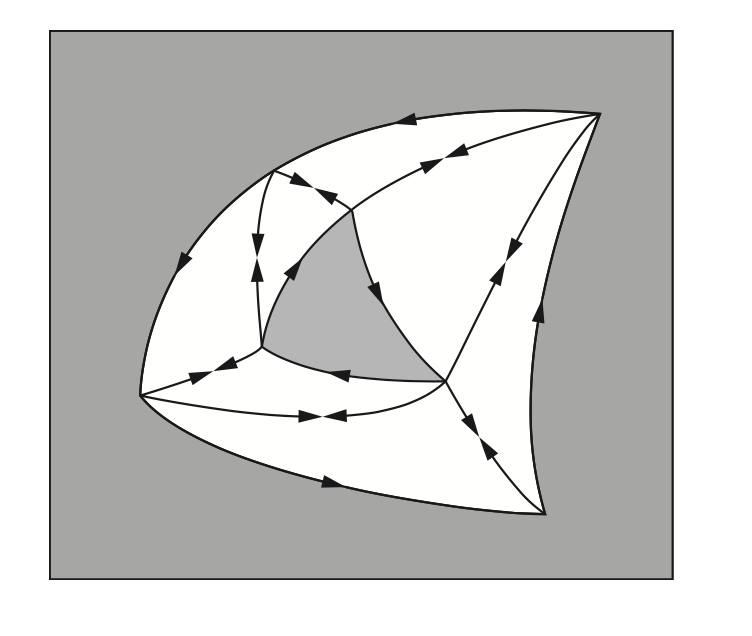
\includegraphics[scale = 0.5]{gauss_bonnet_global.png}}
\end{minipage}
\caption{\scriptsize
\textbf{The proof of Gauss-Bonnet theorem global \citep{do1976differential}}}
\label{fig: gauss_bonnet_global}
\end{figure}

By applying to every triangle the \emph{\textbf{local Gauss-Bonnet theorem}} and adding up the results we obtain, using Proposition \ref{prop: area_integral} and the fact that each "\emph{interior}" side is described \emph{\textbf{twice}} in \emph{\textbf{opposite orientations}},
\begin{align*}
\sum_{i=1}^{n}\int_{C_{i}}k_{g}(s)ds + \iint_{\cR}\mb{K}d\sigma + \sum_{j}^{F}\sum_{k=1}^{3}\theta_{j,k} &= 2\pi\,F
\end{align*} where $F$ denotes the number of triangles of $J$, and $\theta_{j,1}, \theta_{j,2} , \theta_{j,3}$ are the \textbf{\emph{external angles}} of the \emph{triangle} $T_j$.

We shall now introduce the \textbf{\emph{interior angles}} of the triangle $T_j$, given by $\varphi_{j,k} = \pi - \theta_{j,k}$. Thus,
\begin{align*}
\sum_{j}^{F}\sum_{k=1}^{3}\theta_{j,k} &=  \sum_{j}^{F}\sum_{k=1}^{3}\paren{\pi  - \varphi_{j,k}} = 3\pi\,F -  \sum_{j}^{F}\sum_{k=1}^{3}\varphi_{j,k}
\end{align*}
We shall use the following notation:
\begin{itemize}
\item $E_e =$ number of \emph{\textbf{external} edges} of $J$,
\item $E_i =$ number of \emph{\textbf{internal} edges} of $J$,
\item $V_e =$ number of \emph{\textbf{external vertices}} of $J$,
\item $V_i =$ number of \emph{\textbf{internal vertices}} of $J$.
\end{itemize}
Since the curves $C_i$ are \emph{closed}, $E_e = V_e$. Furthermore, it is easy to show by induction that
\begin{align*}
3\,F &= 2\,E_i + E_e
\end{align*}
and therefore that
\begin{align*}
\sum_{j}^{F}\sum_{k=1}^{3}\theta_{j,k} &=  \paren{2\pi\, E_i + \pi E_e} -  \sum_{j}^{F}\sum_{k=1}^{3}\varphi_{j,k}
\end{align*}

We observe now that \emph{the external vertices may be either \textbf{vertices of some curve} $C_i$ or \textbf{vertices introduced by the triangulation}}. We set $V_e = V_{ec} + V_{et}$ , where $V_{ec}$ is the number of vertices of the curves $C_i$ and $V_{et}$ is the number of external vertices of the triangulation which are \emph{\textbf{not vertices of some curve}} $C_i$. Since the \emph{sum of angles} around \emph{each \textbf{internal vertex}} is $2\pi$, we obtain
\begin{align*}
\sum_{j}^{F}\sum_{k=1}^{3}\theta_{j,k} &=  \paren{2\pi\, E_i + \pi E_e} - \paren{2\pi\,V_{i} + \pi\,V_{et}} -  \sum_{i=1}^{p}\paren{\pi - \theta_{i}}
\end{align*}

By adding $\pi E_e$ to and subtracting it from the expression above and taking into consideration that $E_e = V_e$, we conclude that
\begin{align*}
\sum_{j}^{F}\sum_{k=1}^{3}\theta_{j,k} &=  \paren{2\pi\, E_i + 2\pi E_e} - \paren{2\pi\,V_{i} + \pi\,V_e +  \pi\,V_{et} + \pi\,V_{ec}} + \sum_{i=1}^{k}\theta_{i}\\
&= 2\pi\,E - 2\pi\,V + \sum_{i=1}^{p}\theta_{i}.
\end{align*}

By putting things together, we finally obtain
\begin{align*}
\sum_{i=1}^{n}\int_{C_{i}}k_{g}(s)ds + \iint_{\cR}\mb{K}d\sigma + \sum_{i=1}^{p}\theta_{i} &= 2\pi\,\paren{F - E + V}\\
&= 2\pi\,\chi(\cR)
\end{align*} \qed
\end{proof}

\item Note that the Euler-Poincar\'e characteristic of a simple region is $1$, we obtain
\begin{corollary}
If $\cR$ is a \textbf{simple region} of $\cS$, then
\begin{align*}
\sum_{i=1}^{k}\int_{s_{i}}^{s_{i+1}}k_{g}(s)ds + \iint_{\cR}\mb{K}d\sigma + \sum_{i=1}^{k}\theta_{i} &= 2\pi
\end{align*}
\end{corollary}

\item By taking into account the fact that a compact surface may be considered as a region with empty boundary, we obtain
\begin{corollary}\label{thm: total_curvature_invariant}
Let $\cS$ be an orientable \textbf{compact} surface; then
\begin{align*}
\iint_{\cS}\mb{K}d\sigma &= 2\pi\,\chi(\cS)
\end{align*}
\end{corollary}

\begin{remark}\citep{do1976differential}\\
Corollary \ref{thm: total_curvature_invariant} is most striking. We have only to think of all possible shapes of a surface \emph{\textbf{homeomorphic}} to a \textbf{sphere} to find it very surprising that in each case the curvature function distributes itself in such a way that the \emph{\textbf{total curvature}}, i.e. $\iint_{\cR}\mb{K}d\sigma$ is \textbf{\emph{the same for all cases}}.
\end{remark}
\end{itemize}


\section{The Applications}
\begin{itemize}
\item We shall present some applications of the Gauss-Bonnet theorem below. For these applications, it is convenient to assume a basic fact of the \emph{topology of the plane} (\emph{\textbf{the Jordan curve theorem}}) which we shall use in the following form: Every \emph{closed piecewise regular curve} in the \emph{\textbf{plane}} (thus without self-intersections) is the \emph{\textbf{boundary}} of a \emph{\textbf{simple region}}.

\item \begin{proposition} 
A \textbf{compact} surface of \underline{\textbf{positive curvature}} is \textbf{homeomorphic} to a sphere.
\end{proposition}
The Euler-Poincar\'e characteristic of such a surface is \emph{\textbf{positive}} and the \emph{sphere is the \textbf{only} compact surface of $\bR^3$ which satisfies this condition}.

\item \begin{proposition}
Let $\cS$ be an orientable surface of \underline{\textbf{negative or zero curvature}}. Then two geodesics $\gamma_1$ and $\gamma_2$ which start from a point $p \in \cS$ \textbf{cannot meet again} at a point $q \in \cS$ in such a way that the \textbf{traces} of $\gamma_1$ and $\gamma_2$ constitute the \textbf{boundary} of a simple region $\cR$ of $\cS$.
\end{proposition}
\begin{proof}
Assume that the contrary is true. By the Gauss-Bonnet theorem ($\cR$ is simple)
\begin{align*}
\iint_{\cR}\mb{K}d\sigma + \theta_1 + \theta_{2} &= 2\pi
\end{align*}
where $\theta_1$ and $\theta_{2}$ are the \emph{\textbf{external angles}} of the region $\cR$. Since the geodesics $\gamma_1$ and $\gamma_2$ cannot be mutually tangent, we have $\theta_i < \pi$, $i = 1, 2$. On the other hand, $\mb{K} \le 0$, whence the contradiction.


When $\theta_1 = \theta_2 = 0$, the traces of the geodesics $\gamma_1$ and $\gamma_2$ constitute a \emph{simple \textbf{closed} geodesic} of $\cS$ (that is, a \emph{closed regular curve} which is a \emph{geodesic}). It follows that on \emph{a surface of zero or negative curvature}, there exists \emph{no simple closed geodesic} which is a boundary of a simple region of $\cS$. \qed
\end{proof}

\item \begin{proposition}
Let $\cS$ be a surface \textbf{diffeomorphic} (i.e., there exists a differentiable map which has a differentiable inverse) to a \textbf{cylinder} with Gaussian curvature $\mb{K} < 0$. Then $\cS$ has \textbf{at most one} simple \textbf{closed} \textbf{geodesic}.
\end{proposition}
\begin{proof}
Suppose that $\cS$ contains one simple closed geodesic $\Gamma$. By application 2, and since there is a diffeomorphism $\varphi$ of $\cS$ with a plane $P$ minus one point $q \in P$, $\varphi(\Gamma)$ is the boundary of a simple region of $P$ containing $q$.

\begin{figure}[htb]
\centering
\begin{minipage}{1\linewidth}
 \centerline{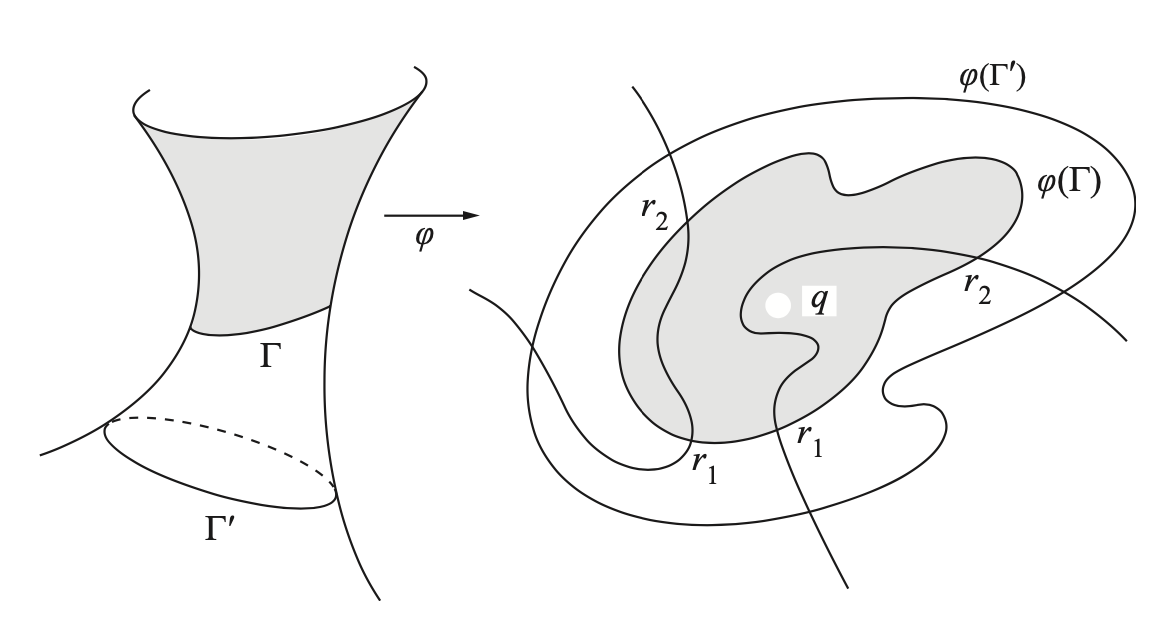
\includegraphics[scale = 0.5]{gauss_bonnet_app_1.png}}
\end{minipage}
\caption{\scriptsize
\textbf{ \citep{do1976differential}}}
\label{fig: gauss_bonnet_app_1}
\end{figure}


Assume now that $\cS$ contains another simple closed geodesic $\Gamma'$. We claim that $\Gamma'$ does not intersect $\Gamma$. Otherwise, the arcs of $\varphi(\Gamma)$ and $\varphi(\Gamma')$ between two "consecutive" intersection points, $r_1$ and $r_2$, would be the boundary of a simple region, contradicting application 2 (see Fig. 4-33). We can now apply the Gauss-Bonnet theorem to the region $\cR$ bounded by two simple, non-intersecting geodesics $\Gamma$. and $\Gamma'$ of $\cS$. Since $\chi(\cR) = 0$, we obtain
\begin{align*}
\iint_{\varphi^{-1}(\cR)}\mb{K}d\sigma &= 2\pi\,\chi(\cR) = 0
\end{align*} which is a contradiction, since $\mb{K} < 0$. \qed
\end{proof}

\item \begin{proposition}
If there exist two simple \textbf{closed} \textbf{geodesics} $\Gamma_1$ and $\Gamma_2$ on a \textbf{compact}, connected surface $\cS$ of \textbf{positive curvature}, then $\Gamma_1$ and $\Gamma_2$  \textbf{intersect}.
\end{proposition}
\begin{proof}
By application 1, $\cS$ is \textbf{homeomorphic} to a sphere. If  $\Gamma_1$ and $\Gamma_2$ do not intersect, then the set formed by  $\Gamma_1$ and $\Gamma_2$ is the boundary of a region $\cR$, the Euler-Poincar\'e characteristic of which is $\chi(\cR) = 0$. By the Gauss-Bonnet theorem,
\begin{align*}
\iint_{\cR}\mb{K}d\sigma &= 2\pi\,\chi(\cR) = 0
\end{align*} which is a contradiction, since $\mb{K} > 0$. \qed
\end{proof}

\item \begin{remark} (\textbf{\emph{Non-Euclidean Geometry}})\\
Let $T$ be a \textbf{geodesic triangle} (that is, the sides of $T$ are \textbf{geodesics}) in an oriented surface $\cS$. Assume that Gauss curvature $\mb{K}$ does not change sign in $T$. Let $\theta_1, \theta_2, \theta_3$ be the \textbf{external angles} of $T$ and let $\varphi_1 = \pi - \theta_1$,  $\varphi_2 = \pi - \theta_2$,  $\varphi_3 = \pi - \theta_3$ be its \textbf{interior angles}. By the Gauss-Bonnet theorem,
\begin{align*}
\iint_{T}\mb{K}d\sigma + \sum_{i=1}^{3}\theta_i &= 2\pi\,
\end{align*}
Thus,
\begin{align}
\iint_{T}\mb{K}d\sigma &= 2\pi- \sum_{i=1}^{3}\theta_i = -\pi + \sum_{i=1}^{3}\varphi_{i} \label{eqn: non_euclidean_sum_interior_angles}
\end{align}
It follows that the sum of the interior angles, $\sum_{i=1}^{3}\varphi_{i}$, of a geodesic triangle is
\begin{enumerate}
\item Equal to $\pi$ if $\mb{K} = 0$. (i.e. \textbf{plane})
\item Greater than $\pi$ if $\mb{K} > 0$. (i.e. \textbf{elliptic}) 
\item Smaller than $\pi$ if $\mb{K} < 0$. (i.e. \textbf{hyperbolic}) 
\end{enumerate}

Furthermore, the difference $\sum_{i=1}^{3}\varphi_{i} - \pi$ (the \emph{\textbf{excess}} of $T$) is given precisely  by $\iint_{T}\mb{K}d\sigma$. If $\mb{K} \neq 0$ on $T$, this is the \emph{\textbf{area} of \textbf{image}} $N(T)$ of $T$ by the \emph{\textbf{Gauss map}} $N: \cS \rightarrow \bS^2$. This was the form in which Gauss himself stated his theorem: 

\emph{\textbf{The excess of a geodesic triangle $T$ is equal to the area of its spherical image $N(T)$}}.

The above fact is related to a historical controversy about the possibility of proving Euclid’s fifth axiom (the axiom of the parallels), from which it follows that the sum of the interior angles of any triangle is equal to $\pi$. 
\end{remark}

\end{itemize}


\newpage
\bibliographystyle{plainnat}
\bibliography{book_reference.bib}
\end{document}